\documentclass[aspectratio=169]{beamer}
\usepackage[T1]{fontenc}
\usepackage[utf8]{inputenc}
\usepackage{amsmath}
\usepackage{amssymb}
\usepackage{animate}
\usepackage{biblatexmods}  % custom biblatex commands
\usepackage{booktabs}  % nice tables
\usepackage{caption}
\usepackage{enumerate}  % enumitem fails: https://tex.stackexchange.com/q/31505/73149
\usepackage{talk}  % custom overrides
% \addbibresource{refs.bib}

% Verbatim size
% See: https://tex.stackexchange.com/a/171866/73149
\makeatletter
\newcommand{\verbatimfont}[1]{\renewcommand{\verbatim@font}{\ttfamily#1}}
\makeatother

% References
% \hypersetup{pdfpagemode=FullScreen}  % always open full screen
\usepackage{hyperref}
\hypersetup{colorlinks,linkcolor=,urlcolor=blue}
\urlstyle{same}
\usepackage[capitalise,noabbrev]{cleveref}  % for pandoc
\creflabelformat{equation}{#2\textup{#1}#3}  % for style
\newcommand{\crefrangeconjunction}{--}

% Graphics
% * Run on command line: convert -coalesce mygif.gif sub/mygif.png
% * Then use: \animategraphics[loop,controls,width=\linewidth]{framerate}{sub/mygif-}{0}{framecount}
%   The \animategraphics will trigger 'compile' function to open in Adobe Reader
\usepackage{graphicx}
\usepackage{epstopdf}
\graphicspath{{./figures/}}
\epstopdfDeclareGraphicsRule{.gif}{png}{.png}{convert gif:#1 png:\OutputFile}
\AppendGraphicsExtensions{.gif}  % convert static gif images to readable format
\newcommand*{\vcenteredhbox}[1]{\begingroup\setbox0=\hbox{#1}\parbox{\wd0}{\box0}\endgroup}

% Presenting. Impressive is limited (no presenter mode, just transitions) and Présentation
% has major issues (shortcuts don't work and aren't read into stdin). Former also
% requires python 2 venv, PIL (conda), PyOpenGL (conda), PyGame (pip), and PDFTK
% (see https://www.pdflabs.com/tools/pdftk-server and https://orinanobworld.blogspot.com/2016/04/solved-problem-with-impressive.html)
% Option A: Comments with Impressive, PymPress, beamer
% \usepackage{pgfpages}
% \setbeameroption{show notes on second screen=right}
% \note{note here}
% Option B: Comments with osx-presentation or Présentation
\usepackage{pdfcomment} % the package
\let\oldpdfcomment\pdfcomment
\renewcommand{\pdfcomment}[1]{\marginnote{\oldpdfcomment[icon=note]{#1}}}  % prevent overlap
% \pdfcomment{comment here}

% Logos
% General: http://jhshi.me/2013/12/02/place-logo-properly-in-beamer/index.html
% Keep at top right: https://bloerg.net/2012/06/21/customizing-the-frametitle-of-beamer-presentation.html
% \usepackage{pgf}  % mysterious magic package
% \logo{\includegraphics[height=40pt]{csulogo1.png}}  % normal
% \logo{\pgfputat{\pgfxy(0,8)}{\pgfbox[right,top]{\includegraphics[width=1.7cm]{csulogo1.png}}}}  % custom position
% \titlebackgroundfile{bgtitle}  % for title pages sections etc.
% \framebackgroundfile{bgframe}  % for framing content of normal pages

% Head
\begin{document}
\title{Introduction to NetCDF}
\author[Davis, Luke]{Luke Davis}
\institute[CSU]{Department of Atmospheric Science\\Colorado State University}
\date{}
\frame{\titlepage}

% Body
\section{Introduction}
\begin{frame}

  \frametitle{Who am I?}

\end{frame}


\begin{frame}

  \frametitle{Background}

  \textbf{Problem}:
  % often
  Earth scientists
  work with
  huge,
  4+ dimensional datasets
  (3 spatial dimensions, 1 time dimension, and sometimes even more).
  % datasets with 4+ dimensions:
  % data
  % work with huge amounts of data in 4+ dimensions:
  %
  \begin{itemize}
    \item
      Example: Air temperature (longitude, latitude, height, time)
    \item
      Example: Surface pressure from ``ensemble'' of model simulations
      (longitude, latitude, time, ensemble member)
    \item
      Example: Satellite-retrieved radiation
      (projection x-coordinate, projection y-coordinate, wavenumber)
  \end{itemize}

\end{frame}


\begin{frame}
  \frametitle{Background}

  \textbf{Question}:
  What's the best way to \textbf{store} this type of data?
  %
  \begin{itemize}
    \item Spreadsheets? Not enough dimensions.
    \item Matrices? No way to annotate ``rows'', ``columns'', etc.
  \end{itemize}
  % How can we

  \textbf{Answer}:
  The \href{https://en.wikipedia.org/wiki/NetCDF}{NetCDF} format (Network Common Data Form)
  developed by \href{https://www.unidata.ucar.edu/software/netcdf/}{UCAR/Unidata}
  (right down the road!).
  %
  \begin{itemize}
    \item
      Description: {\color{red}Annotated} N-dimensional matrices (arrays)
    \item
      File extension: \texttt{.nc}
  \end{itemize}

  There are other similar data formats
  (\href{https://en.wikipedia.org/wiki/Hierarchical_Data_Format}{HDF},
  \href{https://en.wikipedia.org/wiki/GRIB}{GRIB}),
  and some software can work seamlessly with different formats\ldots
  but {\color{red}NetCDF is your new best friend}.
  % (some software can work seamlessly with NetCDF, HDF, GRIB).
  % \textbf{Problem}: How do I store geophysical data
  % (e.g., observations, model output).

\end{frame}


\begin{frame}
  \frametitle{Architecture}

  File formats have
  \href{https://www.unidata.ucar.edu/software/netcdf/docs/faq.html#whatisenhanceddatamodel}{different ``version numbers''}:
  %
  \begin{itemize}
    \item
      NetCDF3 (version 3)
      \href{https://www.unidata.ucar.edu/software/netcdf/docs/RELEASE_NOTES.html#autotoc_md60}{retired in 2008}.
      Unidata is \href{https://www.unidata.ucar.edu/software/netcdf/docs/RELEASE_NOTES.html#autotoc_md0}{currently version 4}.
    \item
      \ldots however version 3 still widespread
      (scientists are slow to change their ways\ldots too many other things to worry about).
    \item
      Some things 
      in NetCDF4 are impossible in NetCDF3
      (multiple unlimited dimensions, \ldots).
    \item
      Weird read/write bugs are sometimes due to version incompatibilities.
  \end{itemize}

  NetCDF3 still everywhere, so you may need to use it.
  % \texttt{\$ ncdump -h example.nc}
\end{frame}

\begin{frame}

  \frametitle{Architecture}

  NetCDF files have the following featuers:
  %
  \begin{itemize}
    \item
      Global attributes.
    \item
      Global dimensions.
    \item
      Named variables, each with its own
      dimensions and attributes.
  \end{itemize}

\end{frame}

\begin{frame}[fragile]

  \frametitle{Architecture}

\begin{verbatim}
$ ncdump -h example.nc
ADD EXAMPLE
\end{verbatim}

\end{frame}



\begin{frame}
  \frametitle{Software}

  % Several types of sotware
  There's lots of sotware for working with NetCDF (HDF, GRIB) files.
  First, the \textbf{command-line} tools:
  %
  \begin{itemize}
    \item
      NCO ({\color{red}N}et{\color{red}C}DF {\color{red}O}perators).
      % Include ``ncdump'' (dump NetCDF file contents)
      % NetCDF operators (``NCO'').
  \end{itemize}

\end{frame}

\begin{frame}
  \frametitle{Software}

  Next, the \textbf{python} tools:
  %
  \begin{itemize}
    \item
      \href{https://unidata.github.io/netcdf4-python/}{netCDF4}
      (confusingly, this works with both Netcdf versions 3 and 4!).
      netCDF4 is for {\color{red}low-level, fast} control.
    \item
      \href{http://xarray.pydata.org/en/stable/}{xarray}
      (``new kid'' on the block but \textit{extremely} powerful).
      xarray is for {\color{red}high-level, convenient} control.
    \item
      Python also has
      \href{https://scitools.org.uk/iris/docs/v1.13.0/userguide/loading_iris_cubes.html}{Iris ``cubes''}\ldots
      but this is older, less widespread, falling out of favor
      (%
      xarray intended as
      \href{http://xarray.pydata.org/en/stable/getting-started-guide/faq.html#what-other-netcdf-related-python-libraries-should-i-know-about}{improvement on ``cubes''}%
      ).
  \end{itemize}
\end{frame}


\section{Command-line tools}

\begin{frame}
\frametitle{CDO Overview}

  Many of us know about NCO
  ({\color{red}N}et{\color{red}C}DF {\color{red}O}perators) and
  NCL ({\color{red}N}CAR {\color{red}C}ommand {\color{red}L}anguage).

  A comparatively recent player is \textbf{CDO}
  ({\color{red}C}limate {\color{red}D}ata {\color{red}O}perators).

  \begin{itemize}
    \item
      Written in C++ by Max Planck Institut. \textbf{Companion} to NCO
    -- does things NCO can't.
    \item
      Install with Anaconda, no sudo necessary:
      \texttt{conda install -c conda-forge cdo=1.9.0}.
    % \item Great documentation. %:
      % \url{https://code.mpimet.mpg.de/projects/cdo/embedded/index.html}.
    \item
      Great documentation, easy-to-remember syntax:
      \texttt{cdo -mergetime 2017*.nc out.nc}.
    \item
      \textbf{Subcommand chaining}:
      \texttt{cdo -add -sqr -selname,u f.nc -sqr -selname,v f.nc \textbf{KE.nc}}.
  \end{itemize}

  \begin{center}
    \vspace{-5pt}
        % \noindent \fbox{\parbox{\textwidth}{%
        \texttt{{\color{red}cdo -zonmean -mul -sub -selname,t f.nc -enlarge,f.nc -zonmean -selname,t f.nc \textbackslash}}\\
        \texttt{{\color{red}-sub -selname,v f.nc -enlarge,f.nc -zonmean -selname,v f.n\textbf{c EHF.nc}}}.
      % }}
    \end{center}
    \begin{itemize}
      % \boxed{\texttt{cdo -zonmean -mul -sub -selname,t f.nc -enlarge,f.nc -zonmean
        % -selname,t f.nc \textbackslash}\\ \texttt{-sub -selname,v f.nc -enlarge,f.nc
        %  -zonmean -selname,v f.nc EHF.nc}}.
        \item
          Reads \textbf{GRIB} and \textbf{NetCDF} files; convert with \texttt{cdo -f nc f.grb f.nc}.
        \item
          \textbf{Streams} input file into output file; does \textbf{not} load entire file into memory.
        \item
          \textbf{{\color{red}Warning}}: For many operations,
          \textbf{dimension attributes matter}!
          Verify CDO is reading your file ``correctly'' with
          \texttt{griddes}, \texttt{zaxisdes}, \texttt{showdate}, \ldots
    % \item Well-written; source code is in C++, and does not load entire files into
      % memory; efficient for \textbf{big} datasets. \item Written in C, released by Max
      % Planck Institut in Germany. \item Efficient for big datasets -- does not load
      % entire file into memory when possible. \item Get temporal trends ignoring NaNs,
      % spatial EOFs, monthly daily and seasonal statistics, convert from GRIB to
      % NetCDF.
    % \item \textbf{Hundreds} of subcommands available! \item Combine and separate out
      % into multiple files, convert from GRIB to NetCDF, rename variables, chain
      % commands together. \item Use python API or write shell scripts. \item Written in
      % C language and does not require loading entire dataset into memory.
  \end{itemize}
\end{frame}

\begin{frame}
  \frametitle{CDO Uses}
  % Awesome special uses:
  \note{Also if you use CDO you'll probably become a bash scripting pro, which makes you
  really fun at parties. So that's a plus.}

  CDO has \textbf{hundreds} of subcommands. Here's a quick survey:
  \begin{itemize}
    \item \textbf{Regrid} from one arbitrary grid (e.g. rotated pole, hexagonal cells) to another; choose from a suite of algorithms: \texttt{cdo remapcon,destination\_grid.txt in.nc out.nc}.
    \pause
    \item Interpolate to different \textbf{vertical levels}: \texttt{cdo intlevel,1000,900,800,700,600,500,400,300,200 in.nc out.nc}
    \pause
    \item \textbf{LLS trends} ignoring missing vals: \texttt{cdo regres -seldate,1980-01-01T00:00:00,2009-12-31T23:59:59 in.nc out.nc}.
    \pause
    \item Monthly daily and seasonal \textbf{statistics}: \texttt{cdo ymonmean in.nc climate.nc}.
    \pause
    \item \textbf{Spatial} operations: \texttt{zonmean}; \texttt{fldmean}; \texttt{mulc,101325 -vertmean -genlevelbounds}.
    \pause
    \item Spatial \textbf{EOFs}: \texttt{cdo eof,10 file.nc evals.nc evecs.nc}.
    \pause
    \item Get \textbf{summary statistics} on your file: \texttt{cdo infon -selname,t -seltimestep,1 file.nc}.
  \end{itemize}
\end{frame}

\begin{frame}
  \frametitle{XArray}
  If you use python, \textbf{XArray $\mathbf{\gg}$ netCDF4}. XArray is to pandas as NetCDF files are to CSV files.
  \begin{itemize}
    \pause
    \item Handy objects: Datasets (entire NetCDF file) and DataArrays (single variable within NetCDF file).
    \pause
    \item Load Dataset with \texttt{d = xr.open\_dataset("file.nc", engine="pynio")}. For GRIB files, use \texttt{xr.open\_dataset("file.grb", engine="pynio")} ({\color{red}python 3 compatibility coming soon}).
      % \begin{itemize}
      %   \item Python 3 compatibility for \texttt{pynio} coming soon.
      % \end{itemize}
    \pause
    \item Operate along dimensions: \texttt{d["variable"].mean(dim="longitude")}.
    \pause
    \item Permute dimensions: \texttt{d.transpose(["time", "latitude", "longitude"])}.
    \pause
    \item Slice dimensions: \texttt{d.sel(lat=slice(0,90))}; \texttt{d.sel(level=850, method="nearest")}; 
    \pause
    \texttt{d.sel(time=slice(np.datetime64("2000-01-01"),np.datetime64("2001-01-01")))}.
    \item Get underlying \texttt{numpy} array: \texttt{d["variable"].values}.
    \pause
    \item Save new NetCDF file: \texttt{d.to\_netcdf("filename.nc")}.
  \end{itemize}
    \pause
    \begin{center}
      \textbf{{\color{red}\texttt{import xarray as xr}}}
    \end{center}
\end{frame}


\begin{frame}[fragile]
  \frametitle{NCL}

  There's another tool I didn't mention\ldots
  % There's also
  the \href{https://www.ncl.ucar.edu}{NCAR Command Language} (NCL).
  This is one of my favorites!
  % This is one of my favorite tools!
  %
  \begin{itemize}
    \item
      MATLAB: Everything is an array.
    \item
      Python: Everything is an object (or dictionary, depending on who you ask).
    \item
      {\color{red}NCL}: Everything is a NetCDF-formatted dataset.
      If you're a geoscientist, this paradigm is pretty awesome.
  \end{itemize}

  Sadly, you should avoid using NCL for two reasons\ldots
  %
  \begin{itemize}
    \item
      NCL \href{https://www.ncl.ucar.edu/Document/Pivot_to_Python/september_2019_update.shtml}{is being deprecated}
      (Unidata developers now focusing on python tools).
    \item
      NCL is very slow\ldots among the slowest tools
      (see \href{https://github.com/lukelbd/atmos-benchmarks}{these simple benchmarks}).
  \end{itemize}
\end{frame}


\begin{frame}[fragile]

  \frametitle{NCL}

  \textbf{Example}: Read XYZT temperature and wind data, save YZT eddy heat flux.

\verbatimfont{\footnotesize}%
\begin{verbatim}
$ ncdump -h input.nc
dimensions:
  time = UNLIMITED ; // (200 currently)
  lev = 60 ;
  lat = 36 ;
  lon = 72 ;
variables:
  ...
  double v(time, lev, lat, lon) ;
    v:long_name = "meridional wind" ;
    v:units = "m/s" ;
  double t(time, lev, lat, lon) ;
    t:long_name = "temperature" ;
    t:units = "K" ;
\end{verbatim}

\end{frame}

\begin{frame}[fragile]

  \frametitle{NCL}

  \textbf{Example}: Read XYZT temperature and wind data, save YZT eddy heat flux.

  \verbatimfont{\footnotesize}%
\begin{verbatim}
$ cat fluxes.ncl
f = addfile("input.nc", "r")
o = addfile("output.nc", "c")
t = f->t
v = f->v
ehf = dim_avg_n( \
  (t - conform(t, dim_avg_n(t, 2), (/0, 1/))) \
  * (v - conform(v, dim_avg_n(v, 2), (/0, 1/))), \
  3 \
)
copy_VarCoords(t(:, :, 0), ehf)
ehf@long_name = "eddy heat flux"
ehf@units = "K*m/s"
o->ehf = ehf
\end{verbatim}

\end{frame}

\begin{frame}[fragile]
  \frametitle{NCL}

  \textbf{Example}: Read XYZT temperature and wind data, save YZT eddy heat flux.

  \verbatimfont{\footnotesize}%
\begin{verbatim}
$ ncl fluxes.ncl
$ ncdump -h output.nc
dimensions:
  time = 200 ;
  lev = 60 ;
  lat = 36 ;
variables:
  ...
  double ehf(time, lev, lat) ;
    ehf:units = "K*m/s" ;
    ehf:long_name = "eddy heat flux" ;
\end{verbatim}

\end{frame}


\begin{frame}[plain]
  % \frametitle{Benchmarks: Laptop}
  \begin{figure}
    \centering
    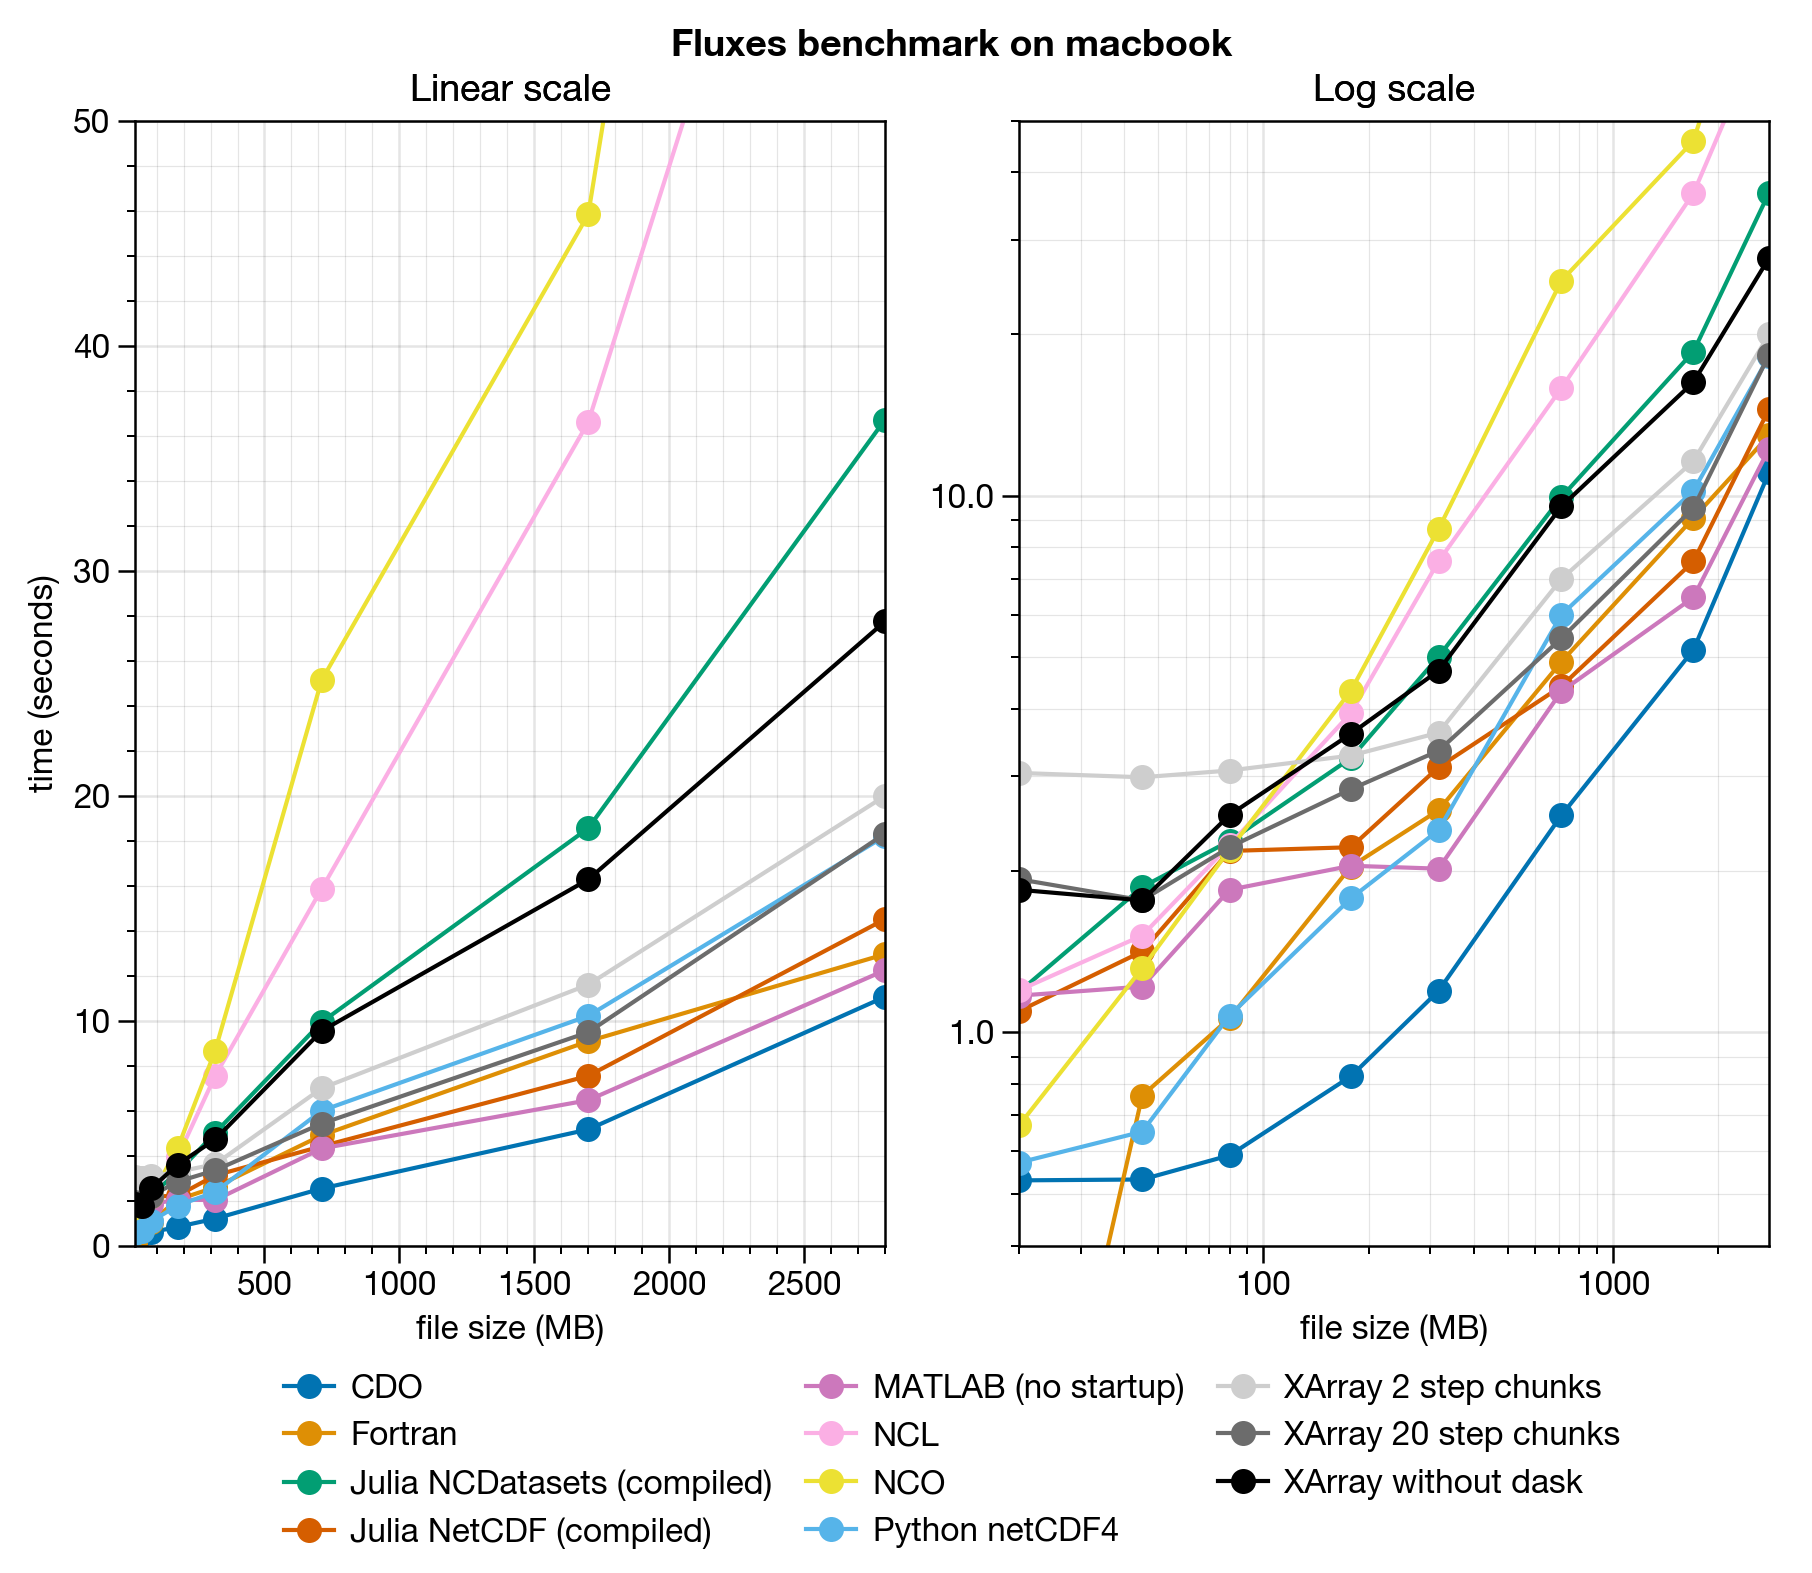
\includegraphics[height=1.1\textheight]{fluxes_60lev_uriah.png}
  \end{figure}
\end{frame}

\begin{frame}[plain]
  % \frametitle{Benchmarks: 72-core supercomputer node}
  \begin{figure}
    \centering
    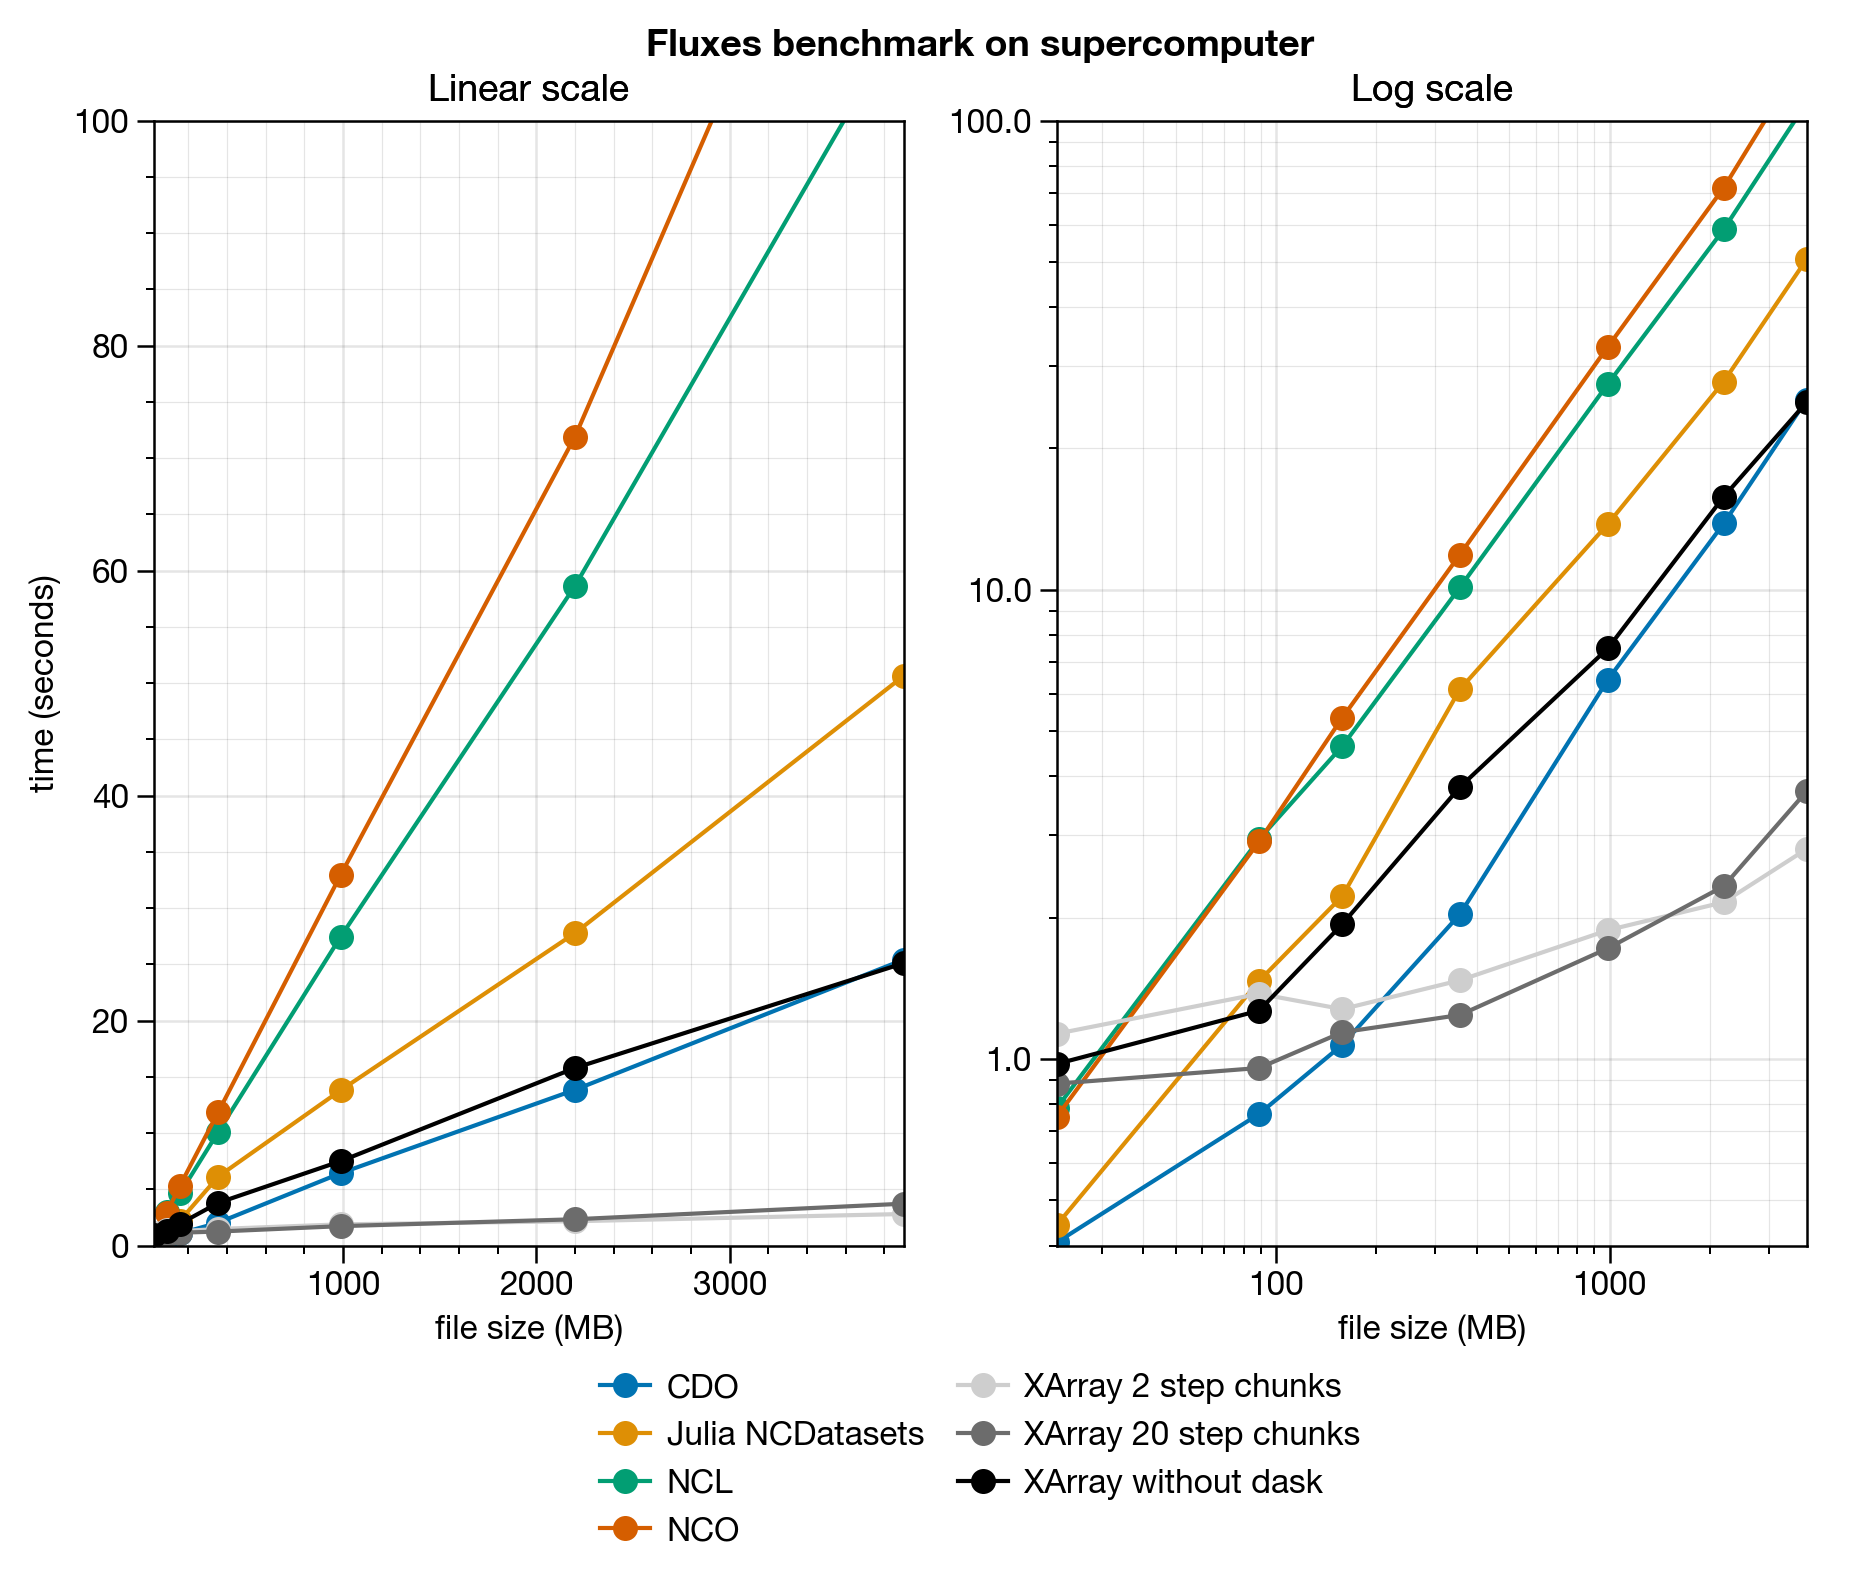
\includegraphics[height=1.1\textheight]{fluxes_60lev_cheyenne4.png}
  \end{figure}
\end{frame}

\begin{frame}[plain]
  % \frametitle{Benchmarks: Simple operations}
  \begin{figure}
    \centering
    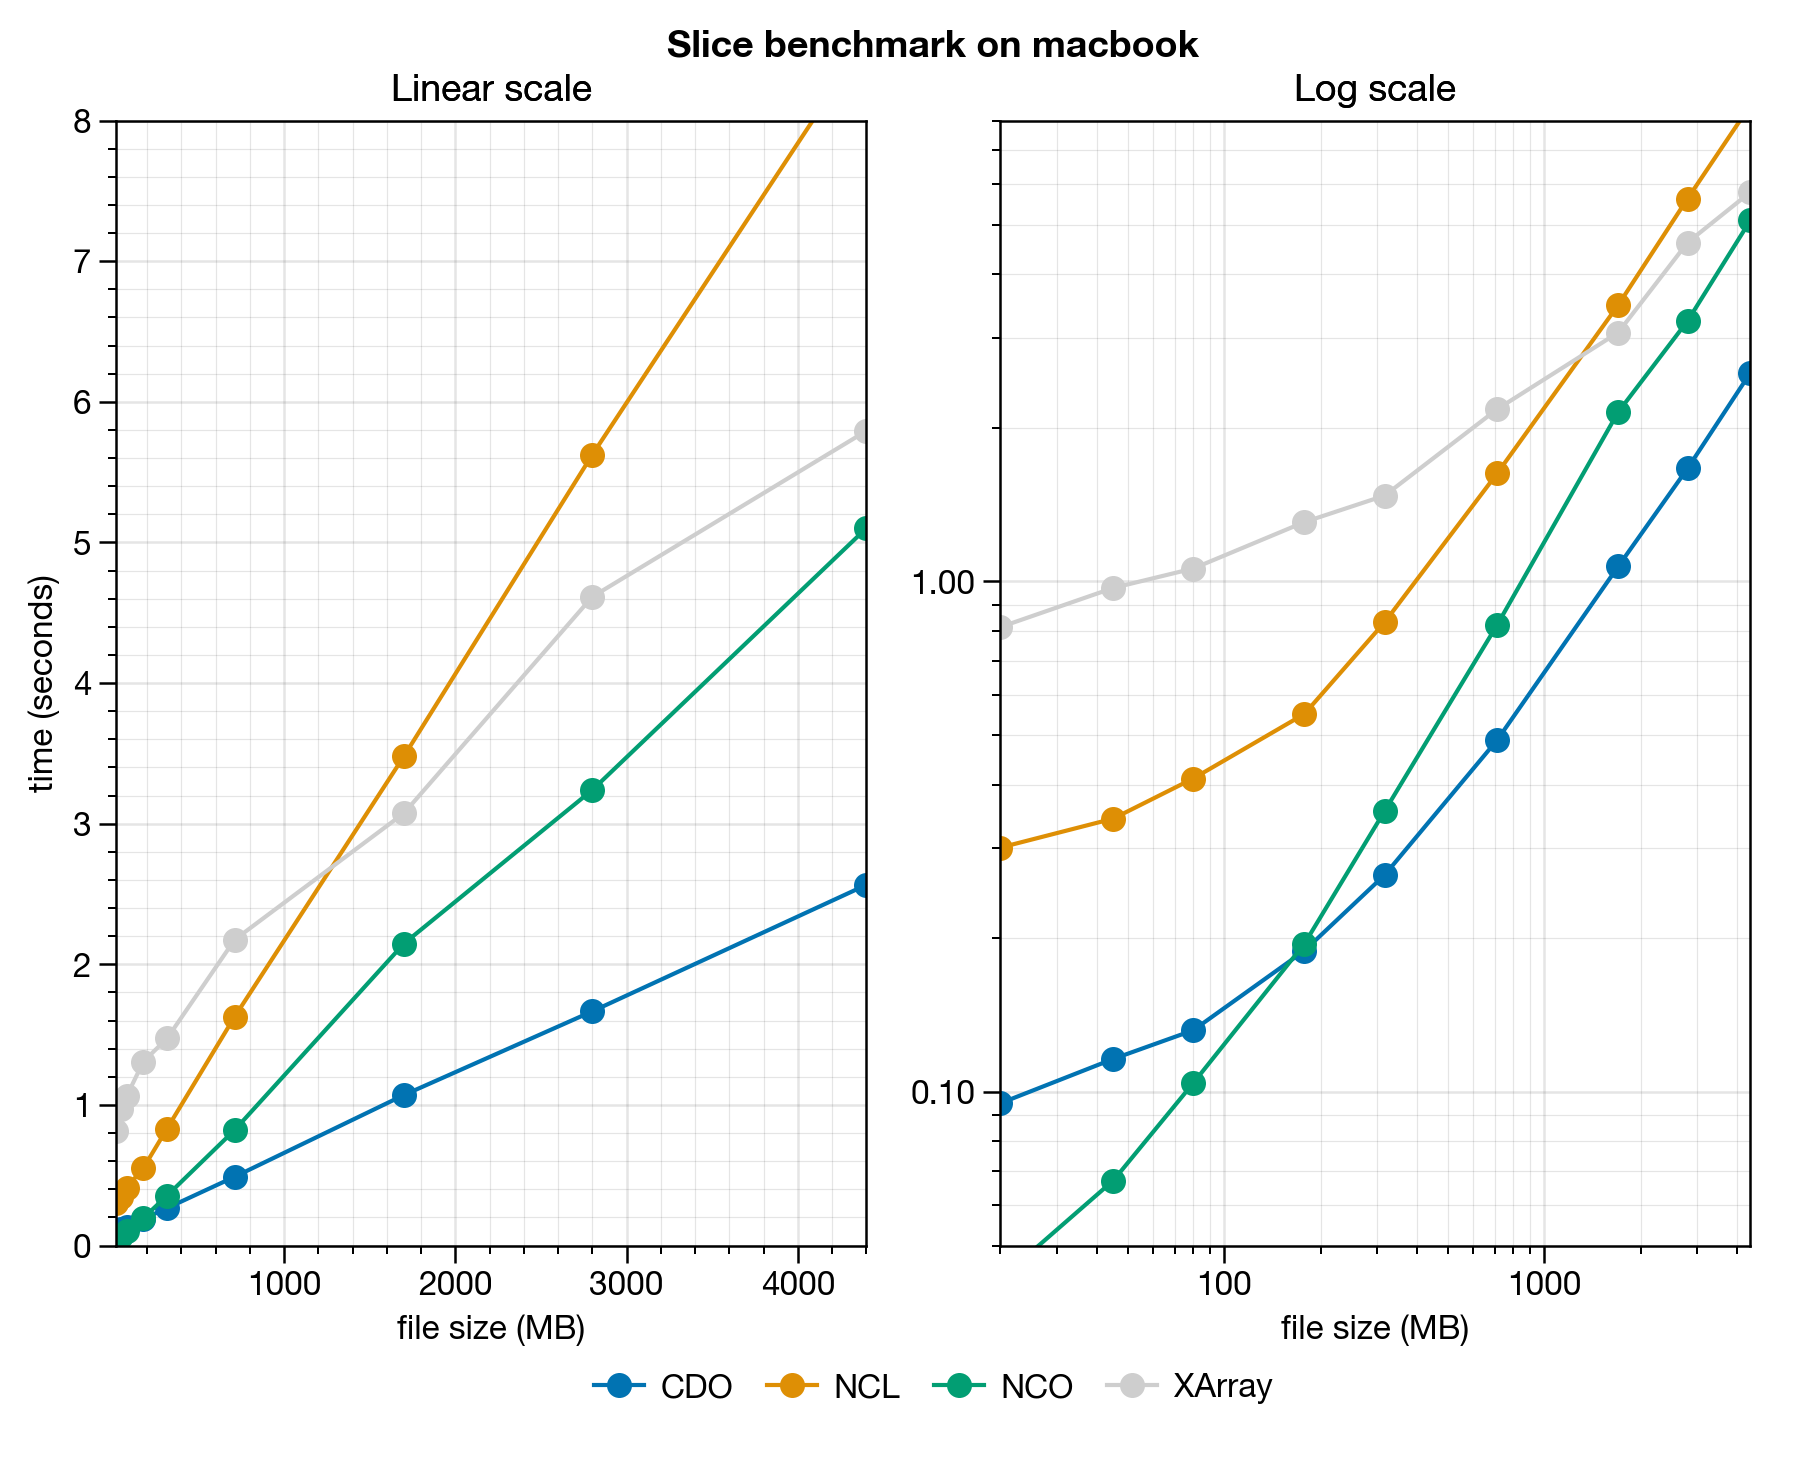
\includegraphics[height=1.1\textheight]{slices_60lev_uriah.png}
  \end{figure}
\end{frame}

\begin{frame}[fragile]
\frametitle{Panoply}
% Climate Data Operators produces output NetCDF files. You often may want to test contents. Panoply is the answer!
Many are familiar with \textbf{ncview}. Modern alternative is \textbf{Panoply}.
  \begin{itemize}
    \item Freeware released by NASA.
    \item Extremely easy to use.
    % \item Make quick plots of data in your NetCDF files.
    % \item Open-source shell utility for manipulating climate-datasets in GRIB and NetCDF. Python API also available.
    % \item Written in C, released by Max Planck Institut in Germany.
    % \item Efficient for big datasets -- does not load entire file into memory when possible.
    % \item Remap from one arbitrary grid to another arbitrary grid, choose from a suite of algorithms.
    % \item Get temporal trends ignoring NaNs, spatial EOFs, monthly daily and seasonal statistics, convert from GRIB to NetCDF.
    % \item \textbf{Hundreds} of subcommands available!
    % % \item Combine and separate out into multiple files, convert from GRIB to NetCDF, rename variables, chain commands together.
    % % \item Use python API or write shell scripts.
    % % \item Written in C language and does not require loading entire dataset into memory.
  \end{itemize}
  \begin{center}
    \vspace{-10pt}
    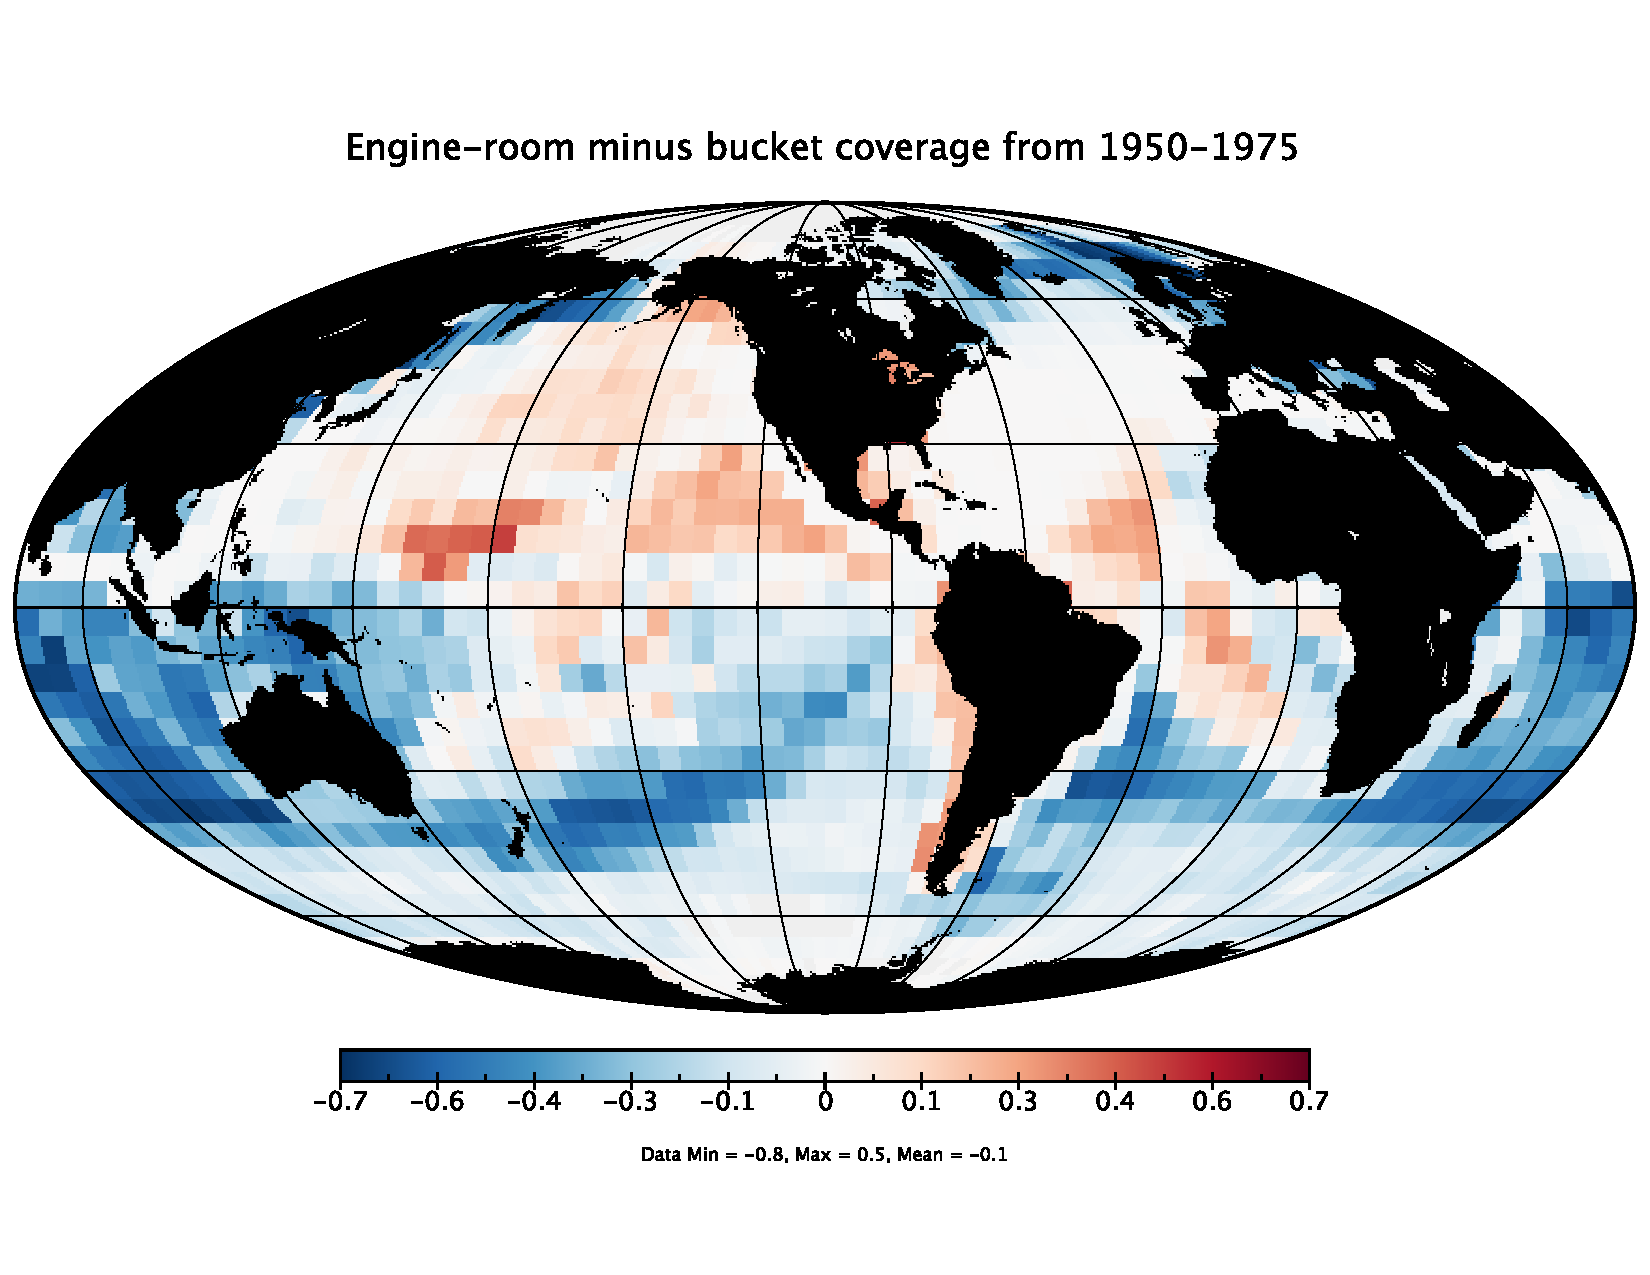
\includegraphics[width=.5\textwidth]{panoply-demo.pdf}
  \end{center}
\end{frame}


\section{Python tools}

\begin{frame}
  \frametitle{netCDF4}

  Now let's get into the python tools.

\end{frame}


\section{Examples}

\begin{frame}
  \frametitle{Learning more}
  \begin{itemize}
    \item
      Use google. Try rephrasing a few times if nothing comes up.
    \item
      Use \href{https://stackoverflow.com}{stackoverflow}!
      \ldots but only \textit{ask} questions after extensive googling fails.

      Tip: For inline-code examples, use \texttt{`inline code'}. For multiline-code
      examples, use \texttt{%
      ```\\
      multiline code\\
      '''%
      }.
    \item
      Use slack!
      Collaboration + cooperation saves everyone time.
      % Waste of time when everyone works on same problem.

      Tip:
      For inline-code and multiline-code, use backticks --
      just like stackoverflow.
  \end{itemize} 
\end{frame}




\end{document}
